% C3: Committed Confidence Calibration -- mid-evaluation slides.
%
%   cd documents/mid-eval-slides
%   ../../.venv/bin/python make_figures.py      # figures/ from artifacts/*.json
%   tectonic slides.tex                          # XeTeX; fetches packages on first run
%
% Every number below is taken from the mid report (documents/DuckDuckDuckGoose-Mid.pdf)
% or from the committed artefacts it was built from. Figures are drawn at their final
% size and included at natural size, so their text matches the slide text.

\documentclass[aspectratio=169,10pt,t]{beamer}

\usefonttheme{professionalfonts}
\usepackage[sfdefault,lining,book,semibold]{FiraSans}
\usepackage[mathrm=sym]{unicode-math}
\setmathfont{FiraMath-Regular.otf}

\usepackage{booktabs}
\usepackage{colortbl}
\usepackage{tabularx}
\usepackage{array}
\usepackage{xspace}
\usepackage{graphicx}
\usepackage{appendixnumberbeamer}
\usepackage{tikz}
\usetikzlibrary{positioning,arrows.meta,calc}
\usepackage[most]{tcolorbox}

\graphicspath{{figures/}}

% ---------------------------------------------------------------- colours
\definecolor{ink}{HTML}{1A1A19}
\definecolor{ink2}{HTML}{52514E}
\definecolor{muted}{HTML}{898781}
\definecolor{gridc}{HTML}{E1E0D9}
\definecolor{base}{HTML}{C3C2B7}
\definecolor{plane}{HTML}{F5F5F2}
\definecolor{accent}{HTML}{2A78D6}
\definecolor{accentdark}{HTML}{1C5CAB}
\definecolor{wash}{HTML}{EEF4FC}
\definecolor{mismatch}{HTML}{FCEAE2}

% ---------------------------------------------------------------- theme
\setbeamersize{text margin left=8mm,text margin right=8mm}
\setbeamertemplate{navigation symbols}{}
\setbeamercolor{normal text}{fg=ink,bg=white}
\setbeamercolor{structure}{fg=accent}
\setbeamercolor{frametitle}{fg=ink}
\setbeamercolor{alerted text}{fg=accentdark}
\setbeamerfont{frametitle}{size=\large,series=\bfseries}
\setbeamerfont{framesubtitle}{size=\small,series=\mdseries}
\setbeamerfont{itemize/enumerate body}{size=\small}
\setbeamerfont{itemize/enumerate subbody}{size=\footnotesize}

\makeatletter
\setbeamertemplate{frametitle}{%
  \vspace*{4mm}%
  {\usebeamerfont{frametitle}\usebeamercolor[fg]{frametitle}\insertframetitle\par}%
  \ifx\insertframesubtitle\@empty\else
    {\vspace{0.6mm}\usebeamerfont{framesubtitle}\color{ink2}\insertframesubtitle\par}%
  \fi
  \vspace{1.4mm}{\color{accent}\rule{10mm}{1.4pt}}\par
}
\makeatother

\setbeamertemplate{footline}{%
  \hbox to \paperwidth{%
    \hspace{8mm}{\color{muted}\fontsize{6.5}{8}\selectfont
      C3 · Committed Confidence Calibration · Mid evaluation}%
    \hfill
    {\color{muted}\fontsize{6.5}{8}\selectfont\insertframenumber\,/\,\inserttotalframenumber}%
    \hspace{8mm}}%
  \vspace{3.5mm}}

\setbeamertemplate{itemize item}{\raisebox{0.18ex}{\color{accent}\rule{0.48em}{0.48em}}}
\setbeamertemplate{itemize subitem}{\color{muted}–}
\setbeamertemplate{enumerate item}{\color{accentdark}\firasemibold\insertenumlabel.}
\setbeamertemplate{itemize/enumerate body begin}{\setlength{\itemsep}{2.6pt}\raggedright}
\setbeamertemplate{itemize/enumerate subbody begin}{\setlength{\itemsep}{1pt}}

% ---------------------------------------------------------------- helpers
\newcommand{\pp}{\,pp\xspace}
\newcommand{\ci}[1]{{\color{ink2}\scriptsize[#1]}}
\newcommand{\fnote}[1]{{\color{ink2}\scriptsize #1\par}}
\newcommand{\lbl}[1]{{\color{accentdark}\firasemibold #1}}
\newcommand{\po}[1]{{\color{muted}\tiny #1}}
\newcommand{\mm}{\cellcolor{mismatch}}
\newcommand{\src}[1]{\par\vfill{\color{muted}\fontsize{6.5}{8}\selectfont #1}\par\vspace{1.2mm}}
\newcolumntype{L}{>{\raggedright\arraybackslash}X}

\newtcolorbox{takeaway}[1][]{enhanced, colback=wash, colframe=wash, boxrule=0pt,
  arc=1.2mm, left=3mm, right=3mm, top=1.2mm, bottom=1.2mm,
  borderline west={1.6pt}{0pt}{accent}, fontupper=\small,
  before upper=\raggedright, #1}

\newtcolorbox{panel}[1][]{enhanced, colback=white, colframe=base, boxrule=0.5pt,
  arc=1.2mm, left=2.4mm, right=2.4mm, top=1.4mm, bottom=1.4mm, fontupper=\footnotesize,
  before upper=\raggedright, #1}

\newcommand{\paneltitle}[1]{{\color{accentdark}\small\firasemibold #1}\par\vspace{0.8mm}}

% big-number tile: value, label
\newcommand{\stat}[2]{%
  \begin{minipage}[t]{\linewidth}\raggedright
    {\fontsize{21}{23}\selectfont\firasemibold #1}\par\vspace{1.2mm}
    {\footnotesize\color{ink2}#2}
  \end{minipage}}

% progress glyph: fraction in [0,1]
\newcommand{\hb}[1]{\tikz[baseline=-0.65ex]{%
  \draw[accent, line width=0.6pt] (0,0) circle (0.8ex);
  \ifdim#1pt>0pt
    \fill[accent] (0,0) -- (90:0.8ex) arc[start angle=90, delta angle=-360*#1, radius=0.8ex] -- cycle;
  \fi}}

\newcommand{\sectionslide}[3]{%
  \begin{frame}[c,plain]
    \hspace*{4mm}\begin{minipage}{0.86\linewidth}\raggedright
      {\color{accent}\fontsize{10}{12}\selectfont\firasemibold #1}\par\vspace{2mm}
      {\fontsize{22}{26}\selectfont\firasemibold #2}\par\vspace{3mm}
      {\color{accent}\rule{14mm}{1.6pt}}\par\vspace{3mm}
      {\color{ink2}\normalsize #3}
    \end{minipage}
  \end{frame}}

\title{C3: Committed Confidence Calibration}
\author{Abhiraj Ratna · Ayush SM · Ojas Kataria · Parth Sharma}

\begin{document}

% ================================================================ 1 title
\begin{frame}[c,plain]
  \hspace*{4mm}\begin{minipage}{0.9\linewidth}\raggedright
    {\color{accent}\fontsize{9.5}{12}\selectfont\firasemibold MID EVALUATION · ANLP MONSOON 2026}\par
    \vspace{4mm}
    {\fontsize{24}{28}\selectfont\firasemibold C3: Committed Confidence\\[1mm] Calibration}\par
    \vspace{3mm}
    {\color{ink2}\large Selection bias in confidence-based token commitment\\[0.6mm]
      in diffusion language models}\par
    \vspace{5mm}
    {\color{accent}\rule{14mm}{1.6pt}}\par
    \vspace{5mm}
    {\normalsize Abhiraj Ratna · Ayush SM · Ojas Kataria · Parth Sharma}\par
    \vspace{1.2mm}
    {\small\color{ink2}Team DuckDuckDuckGoose}
  \end{minipage}
\end{frame}

% ================================================================ 2 motivation
\begin{frame}{Diffusion LMs commit the tokens they are most confident about}
  \framesubtitle{One forward pass scores every masked position; the decoder keeps the top-$k$}
  \vspace{0.5mm}
  \begin{columns}[T,onlytextwidth]
    \begin{column}{0.56\textwidth}
      \centering
      \begin{tikzpicture}[x=0.98cm, y=0.8cm,
          tok/.style={draw=base, line width=0.5pt, rounded corners=1.5pt,
            minimum width=0.86cm, minimum height=0.52cm, inner sep=0pt, font=\footnotesize},
          obs/.style={tok, fill=plane, text=ink},
          msk/.style={tok, fill=white, text=muted},
          win/.style={tok, fill=wash, draw=accent, line width=0.8pt, text=ink}]
        \node[obs] at (1,2.7) {The};
        \node[win] at (2,2.7) {[M]};
        \node[msk] at (3,2.7) {[M]};
        \node[obs] at (4,2.7) {on};
        \node[win] at (5,2.7) {[M]};
        \node[msk] at (6,2.7) {[M]};
        \node[msk] at (7,2.7) {[M]};
        \node[obs] at (8,2.7) {.};
        \foreach \x in {2,5} \node[font=\scriptsize\firasemibold, text=accentdark] at (\x,3.24) {commit};
        \draw[base, line width=0.5pt] (0.5,0) -- (8.5,0);
        \foreach \x/\c/\w/\col in {2/0.91/cat/accent, 3/0.42/sat/base, 5/0.97/the/accent,
                                   6/0.30/red/base, 7/0.77/mat/base} {
          \fill[\col] (\x-0.17,0) rectangle (\x+0.17,{1.85*\c});
          \node[font=\scriptsize, text=ink] at (\x,{1.85*\c+0.17}) {\c};
          \node[font=\footnotesize\itshape, text=ink2] at (\x,-0.25) {\w};
        }
        \node[font=\scriptsize, text=muted, anchor=west] at (0.4,-0.68)
          {candidate $v_i$ with confidence $c_i = \max_v p_\theta(v \mid x_{\mathrm{obs}})$; top $k = 2$ committed};
      \end{tikzpicture}
    \end{column}
    \begin{column}{0.41\textwidth}
      \begin{itemize}
        \item LLaDA-8B and Dream-7B keep the most confident positions (MaskGIT-style);
              Fast-dLLM puts one global threshold on the same number.
        \item A committed token \alert{won}: its confidence was the largest of $m$ noisy
              estimates. That is the setting of the \alert{winner's curse}
              (Efron 2011; Andrews et al.\ 2024).
      \end{itemize}
    \end{column}
  \end{columns}
  \vspace{2mm}
  \begin{takeaway}
    \textbf{Question.} Once a token has won, is its confidence still an honest probability of
    being right? Threshold papers report speed and quality, never calibration.
  \end{takeaway}
\end{frame}

% ================================================================ 3 two error sources
\begin{frame}{Two separate ways parallel decoding goes wrong}
  \framesubtitle{For a set $S$ committed in one step, given the observed context $x_{\mathrm{obs}}$}
  \vspace{-2.5mm}
  \[
    \mathrm{KL}\Big(p^{*} \,\Big\|\, \prod_{i\in S} p_{\theta,i}\Big)
    \;=\; \underbrace{\mathrm{TC}(x_S \mid x_{\mathrm{obs}})}_{\text{(A) dependency}}
    \;+\; \underbrace{\sum_{i\in S} \mathrm{KL}\big(p^{*}_i \,\big\|\, p_{\theta,i}\big)}_{\text{(B) estimation}}
  \]
  \vspace{-1mm}
  \begin{columns}[T,onlytextwidth]
    \begin{column}{0.4\textwidth}
      \begin{itemize}
        \item \textbf{(A)} Marginals, never the joint: tokens can each be plausible yet
              jointly nonsensical.
        \item \textbf{(B)} The marginals themselves are wrong. The dependency literature
              treats (B) as fixed.
        \item Selecting on a noisy estimate is one way (B) could be large
              \alert{exactly where a decoder commits}.
      \end{itemize}
    \end{column}
    \begin{column}{0.57\textwidth}
      \scriptsize
      \renewcommand{\arraystretch}{1.12}
      \arrayrulecolor{base}
      \begin{tabularx}{\linewidth}{@{}p{2.9cm} >{\centering\arraybackslash}X >{\centering\arraybackslash}X@{}}
        \toprule
        {\color{ink2}Work} & {\color{ink2}Calibrated under selection?} & {\color{ink2}Separates (A) and (B)?} \\
        \midrule
        Fast-dLLM; OSDT             & no              & no \\
        KLASS; SWD; LESS            & no              & no \\
        PC-Sampler                  & positional only & no \\
        DAPD; DEMASK; PUNT          & no              & (A) only \\
        ParallelBench               & no              & (A) only \\
        Tang et al.\ (2026)         & no              & identifies \\
        \rowcolor{wash}
        \textbf{This work}          & \textbf{yes}    & \textbf{both} \\
        \bottomrule
      \end{tabularx}
    \end{column}
  \end{columns}
\end{frame}

% ================================================================ 4 propositions
\begin{frame}{Our proposal's argument was wrong; the fix sharpens the question}
  \framesubtitle{State $s$: a document with masked set $M$. Teacher forcing makes correctness $a_i = \mathbb{1}\{v_i = x_{0,i}\}$ observable}
  \vspace{1.5mm}
  \begin{columns}[T,onlytextwidth]
    \begin{column}{0.485\textwidth}
      \begin{panel}[height=36mm]
        \paneltitle{Proposition 1 · Winning adds nothing given confidence and context}
        If the pairs $(\ell_j, a_j)$ are independent across $j \in M$ given $s$, and the pool
        $P$ is drawn independently of them, the winner $i$ of $P$ satisfies
        \[
          \Pr\big(a_i = 1 \mid \ell_i,\, s,\, i = \arg\max_{j\in P} \ell_j\big) = \pi(\ell_i, s).
        \]
        \fnote{However unequal the noise scales: heteroskedastic noise alone cannot bias
        committed confidence.}
      \end{panel}
    \end{column}
    \begin{column}{0.485\textwidth}
      \begin{panel}[height=36mm]
        \paneltitle{Proposition 2 · Exact split of the committed-token gap}
        \[
          \Delta(m) =
          \underbrace{\mathbb{E}_m[\sigma(\ell) - \pi(\ell)]}_{\text{own miscalibration}}
          + \underbrace{\mathbb{E}_m[\pi(\ell) - \pi(\ell, s)]}_{\text{field term}}
        \]
        \fnote{$\pi(\ell)$: ordinary calibration curve; $\pi(\ell,s)$: its context-aware
        version. At $m = 1$ winners are random, so the field term is exactly 0.}
      \end{panel}
    \end{column}
  \end{columns}
  \vspace{2.5mm}
  \begin{takeaway}
    The field term is nonzero only when accuracy at fixed confidence depends on context: the
    \textbf{winner's curse in a corrected, testable form}. Found in simulation, before any
    GPU time; proofs in the backup.
  \end{takeaway}
\end{frame}

% ================================================================ 5 estimands
\begin{frame}{What we measure, and when we declare an effect}
  \framesubtitle{Sign: confidence $-$ accuracy, so positive means overconfident (the proposal used the opposite)}
  \vspace{1.5mm}
  \begin{columns}[T,onlytextwidth]
    \begin{column}{0.315\textwidth}
      \begin{panel}[height=25mm]
        \paneltitle{E1 · committed-token gap}
        $\Delta(m) = \mathbb{E}_m[c_i - a_i]$ over tokens that win pools of size
        $m \in \{1, 2, 4, \dots, 32\}$. Primary contrast $\Delta(32) - \Delta(1)$, read
        beside ECE.
      \end{panel}
    \end{column}
    \begin{column}{0.315\textwidth}
      \begin{panel}[height=25mm]
        \paneltitle{E2 · field effect}
        Observed $\Delta(m)$ minus the gap predicted by $\hat\pi(\ell)$, which sees only the
        token's own confidence. A context-aware $\hat\pi(\ell, s)$ should close the rest.
      \end{panel}
    \end{column}
    \begin{column}{0.315\textwidth}
      \begin{panel}[height=25mm]
        \paneltitle{E3 · trajectory shift}
        Training uses uniform masks; decoders fill easy positions first. Are decoder states
        less calibrated at equal confidence and matched mask rate?
      \end{panel}
    \end{column}
  \end{columns}
  \vspace{2.5mm}
  \begin{columns}[T,onlytextwidth]
    \begin{column}{0.5\textwidth}
      \small\raggedright
      \textbf{Hypotheses.} \lbl{H1} $\Delta(32) - \Delta(1) > 0$;
      \lbl{H2} field term at $m = 32$ is positive;
      \lbl{H3} decoder states are more overconfident than uniform ones.\par\vspace{1.5mm}
      \textbf{Declare rule.} The 95\% interval excludes zero \emph{and} the estimate exceeds
      twice the non-determinism floor. $\delta_{\min} = 0.02$, fixed in advance, sets power.
    \end{column}
    \begin{column}{0.47\textwidth}
      \small\raggedright
      \textbf{Diagnostics} kept from the proposal, fitted on winning tokens:
      \[
        \Pr(a_i{=}1) = \sigma\big(\alpha\,[+\alpha_s] + f(\ell_i) + \beta_z z_{r,m}\big),
      \]
      or rank dummies $\gamma_k$ in place of $z_{r,m}$. State effects $\alpha_s$ absorb the
      field term: $\beta_z < 0$ without them and $\approx 0$ with them signals a field effect.
    \end{column}
  \end{columns}
\end{frame}

% ================================================================ 6 contributions
\begin{frame}{Three contributions on three models}
  \vspace{2mm}
  \begin{columns}[T,onlytextwidth]
    \begin{column}{0.315\textwidth}
      \begin{panel}[height=29mm]
        {\color{accent}\fontsize{16}{18}\selectfont\firasemibold C1}\par\vspace{0.8mm}
        \paneltitle{Selection-conditional calibration audit}
        On a 110M masked diffusion LM we train ourselves (so we control its training data),
        LLaDA-8B and Dream-7B.
      \end{panel}
    \end{column}
    \begin{column}{0.315\textwidth}
      \begin{panel}[height=29mm]
        {\color{accent}\fontsize{16}{18}\selectfont\firasemibold C2}\par\vspace{0.8mm}
        \paneltitle{Both terms of the KL split}
        Exactly, in nats, on a synthetic JSON probe where $p^{*}$ is known; as identified
        contrasts on real text.
      \end{panel}
    \end{column}
    \begin{column}{0.315\textwidth}
      \begin{panel}[height=29mm]
        {\color{accent}\fontsize{16}{18}\selectfont\firasemibold C3}\par\vspace{0.8mm}
        \paneltitle{A recalibration that costs nothing}
        Uses only quantities the decoder already computes: no extra forward passes. It now
        runs whatever C1 finds.
      \end{panel}
    \end{column}
  \end{columns}
  \vspace{3mm}
  \begin{takeaway}
    \textbf{What changed since the proposal.} Simulating its argument showed it needed
    correcting (Proposition 1). The primary endpoints moved from the coefficient $\beta_z$ to
    the gap $\Delta(m)$ and its field term; $\beta_z$ stays as a diagnostic, fitted with and
    without state fixed effects.
  \end{takeaway}
\end{frame}

% ================================================================ 7 instrument
\begin{frame}{The measurement instrument: collect once, analyse many times}
  \vspace{2.5mm}
  \centering
  \begin{tikzpicture}[
      box/.style={draw=base, line width=0.5pt, rounded corners=1.5pt, fill=white,
        text width=3.0cm, minimum height=1.12cm, align=left, inner sep=1.4mm,
        font=\scriptsize, text=ink2},
      gpu/.style={box, fill=wash, draw=accent!45},
      arr/.style={-{Stealth[length=1.6mm]}, line width=0.6pt, color=muted},
      node distance=3.9mm]
    \node[gpu] (a) {{\footnotesize\firasemibold\color{ink} Held-out document}\\FineWeb-Edu, 256 tokens; the true $x_0$ is known};
    \node[gpu, right=of a] (b) {{\footnotesize\firasemibold\color{ink} Mask state $s$}\\uniform rate $t$; decoder-induced (teacher-forced); matched uniform};
    \node[gpu, right=of b] (c) {{\footnotesize\firasemibold\color{ink} One forward pass}\\LLaDA-8B, Dream-7B or our 110M};
    \node[gpu, right=of c] (d) {{\footnotesize\firasemibold\color{ink} One row per (state, position)}\\$v_i, c_i, \ell_i, a_i$, $p$(true), entropy, margin, top-20};
    \node[box, below=8mm of a] (e) {{\footnotesize\firasemibold\color{ink} Draw pools}\\$m \in \{1,\dots,32\}$, 20 pools per state};
    \node[box, right=of e] (f) {{\footnotesize\firasemibold\color{ink} Rank by $\ell$}\\random tie-breaks; keep the top four ranks};
    \node[box, right=of f] (g) {{\footnotesize\firasemibold\color{ink} Estimators}\\$\Delta(m)$, field term, $\beta_z$, $\gamma_k$, residual ICC};
    \node[box, right=of g] (h) {{\footnotesize\firasemibold\color{ink} Inference}\\cross-fitted halves; 10,000 document-bootstrap resamples};
    \draw[arr] (a) -- (b); \draw[arr] (b) -- (c); \draw[arr] (c) -- (d);
    \draw[arr] (d.south) -- ++(0,-3.6mm) -| (e.north);
    \draw[arr] (e) -- (f); \draw[arr] (f) -- (g); \draw[arr] (g) -- (h);
    \node[anchor=south west, font=\tiny\firasemibold, text=accentdark, inner sep=0.8mm] at (a.north west) {COLLECT ONCE · GPU};
    \node[anchor=north west, font=\tiny\firasemibold, text=ink2, inner sep=0.8mm] at (e.south west) {ANALYSE MANY TIMES · CPU · ANY POOL DESIGN};
  \end{tikzpicture}
  \par\vspace{1.5mm}\raggedright
  \begin{columns}[T,onlytextwidth]
    \begin{column}{0.485\textwidth}
      \begin{itemize}\footnotesize
        \item \textbf{Decoder-induced masks} fill each commit with the true token: the
              states an always-right decoder visits, with no knock-on errors.
        \item \textbf{Position-level storage}: about 4M rows for the corpus, not hundreds
              of millions.
      \end{itemize}
    \end{column}
    \begin{column}{0.485\textwidth}
      \begin{itemize}\footnotesize
        \item \textbf{Cross-fitting}: calibrators and the 9-knot spline are fitted on one
              document half; numbers come from the other.
        \item \textbf{Random tie-breaks}: low precision saturates confidence; array order
              must not pick winners.
      \end{itemize}
    \end{column}
  \end{columns}
\end{frame}

% ================================================================ 8 data
\begin{frame}{Data: held-out text with ground truth at every position}
  \vspace{1mm}
  \begin{columns}[T,onlytextwidth]
    \begin{column}{0.5\textwidth}
      \begin{itemize}
        \item \textbf{2,000 calibration documents}, reservoir-sampled from FineWeb-Edu
              (fixed seed, $\geq$ 1,200 characters) and excluded from our 110M's training
              stream; \textbf{500 reserve documents} for the pilot.
        \item \textbf{50/50 document split}: calibrators, splines and C3 fitted on half 1;
              every reported number from half 2.
        \item Regenerated off-cluster: a \textbf{byte-identical} manifest.
        \item \textbf{Tasks}: GSM8K (1,319) and MBPP (500) as teacher-forced documents;
              HumanEval (164) for end-task evaluation only.
      \end{itemize}
    \end{column}
    \begin{column}{0.46\textwidth}
      {\small\textbf{Contamination screen (T4)}}\par
      \vspace{1mm}
      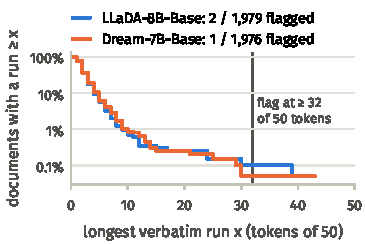
\includegraphics{contamination}\par
      \vspace{0.5mm}
      \fnote{Prompt with the first 50 tokens, generate 50 greedily, take the longest verbatim
      match. Median run: 1 token. The threshold of 32 must be pre-registered before flagged
      documents enter any analysis.}
    \end{column}
  \end{columns}
\end{frame}

% ================================================================ 9 section
\sectionslide{EVALUATIONS SO FAR}{Validate the instrument,\\ then point it at a model}{%
  \small\begin{tabular}{@{}l@{\hspace{6mm}}l@{\hspace{6mm}}l@{}}
    1 · estimator on known truth & 3 · determinism & 5 · power \\[0.6mm]
    2 · four simulated worlds (T0) & 4 · LLaDA-8B-Base pilot (T2) & 6 · our 110M model
  \end{tabular}}

% ================================================================ 10 eval 1
\begin{frame}{Evaluation 1: the regression estimator on known truth}
  \framesubtitle{Eq.~2 on synthetic traces (60 docs × 256 positions, 3 seeds) before any model was touched}
  \vspace{2mm}
  \begin{columns}[T,onlytextwidth]
    \begin{column}{0.68\textwidth}
      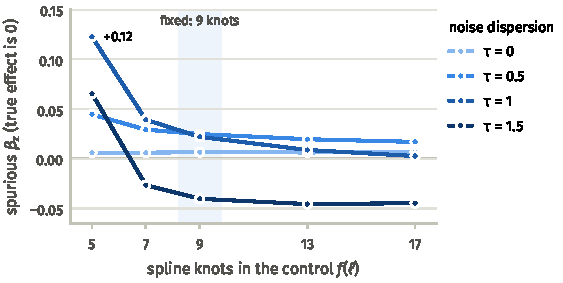
\includegraphics{estimator_validation}\par
      \vspace{0.5mm}
      \fnote{Heteroskedastic null: the noise scale varies across positions with dispersion
      $\tau$, and there is no rank effect, so every nonzero $\beta_z$ is spurious.}
    \end{column}
    \begin{column}{0.29\textwidth}
      \vspace{1mm}
      \footnotesize
      \renewcommand{\arraystretch}{1.1}
      \arrayrulecolor{base}
      \begin{tabularx}{\linewidth}{@{}L r@{}}
        \toprule
        {\color{ink2}Planted $\beta_z$} & {\color{ink2}Recovered} \\
        \midrule
        0 (null)  & $-0.017$ \\
        $-0.10$   & $-0.061$ \\
        $-0.30$   & $-0.242$ \\
        \bottomrule
      \end{tabularx}
      \par\vspace{2mm}
      \begin{itemize}\footnotesize
        \item Planted effects come back smaller: \textbf{conservative}.
        \item 5 knots give a \textbf{spurious $+0.12$} at $\tau = 1$.
        \item \lbl{Decision:} 9 knots fixed in advance (5, 13 as sensitivity);
              $\beta_z$ demoted to a diagnostic.
      \end{itemize}
    \end{column}
  \end{columns}
\end{frame}

% ================================================================ 11 eval 2: T0
\begin{frame}{Evaluation 2 (T0): the endpoints tell four simulated worlds apart}
  \framesubtitle{200 simulated documents · fit half $\rightarrow$ report half · 10,000 document-bootstrap resamples}
  \vspace{1mm}
  \centering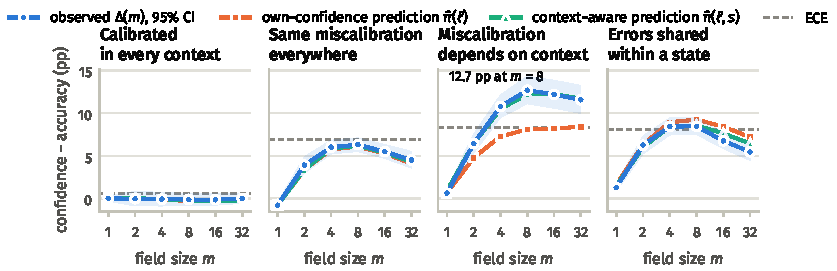
\includegraphics{t0_scenarios}\par
  \vspace{1.5mm}\raggedright
  \begin{takeaway}
    \textbf{Why ECE is not enough.} With context-dependent miscalibration, ECE is 8.3\pp but a
    token that beat 8 candidates is \textbf{12.7\pp} overconfident; own confidence predicts
    8.1, context recovers 12.2.
  \end{takeaway}
\end{frame}

% ================================================================ 12 T0 scorecard
\begin{frame}{T0 scorecard: what the plan expected, and what came out}
  \framesubtitle{$\Delta$ and field term in pp, $\beta_z$ in log-odds, with 95\% intervals. Shaded: observed sign differs from the plan}
  \vspace{1.5mm}
  \scriptsize
  \renewcommand{\arraystretch}{1.0}
  \arrayrulecolor{base}
  \begin{tabularx}{\linewidth}{@{}L c c c c@{}}
    \toprule
    {\color{ink2}Simulated world} & {\color{ink2}$\Delta(32) - \Delta(1)$} & {\color{ink2}Field term, $m = 32$}
      & {\color{ink2}$\beta_z$, no FE} & {\color{ink2}$\beta_z$, with FE} \\
    \midrule
    Calibrated in every context
      & 0.0 \ci{−0.7, +0.7} & \mm +0.1 \ci{+0.1, +0.1} & +0.010 \ci{−0.055, +0.080} & +0.005 \ci{−0.061, +0.076} \\
    \po{\quad plan / observed} & \po{no / no} & \mm\po{0 / $>0$} & \po{0 / 0} & \po{0 / 0} \\[1pt]
    Same miscalibration everywhere
      & +5.3 \ci{+4.4, +6.3} & \mm +0.2 \ci{+0.2, +0.3} & −0.006 \ci{−0.066, +0.056} & −0.004 \ci{−0.066, +0.058} \\
    \po{\quad plan / observed} & \po{yes / yes} & \mm\po{0 / $>0$} & \po{0 / 0} & \po{0 / 0} \\[1pt]
    \textbf{Miscalibration depends on context}
      & +10.9 \ci{+9.5, +12.4} & +3.3 \ci{+2.2, +4.4} & \textbf{−0.246} \ci{−0.305, −0.184} & \mm +0.062 \ci{+0.001, +0.126} \\
    \po{\quad plan / observed} & \po{yes / yes} & \po{$>0$ / $>0$} & \po{$<0$ / $<0$} & \mm\po{0 / $>0$} \\[1pt]
    Errors shared within a state
      & +4.2 \ci{+3.2, +5.3} & −0.7 \ci{−0.9, −0.5} & \mm +0.095 \ci{+0.034, +0.156} & \mm +0.030 \ci{−0.033, +0.093} \\
    \po{\quad plan / observed} & \po{yes / yes} & \po{? / $<0$} & \mm\po{$<0$ / $>0$} & \mm\po{$\neq 0$ / 0} \\
    \bottomrule
  \end{tabularx}
  \vspace{3mm}
  \begin{takeaway}
    $\Delta(32) - \Delta(1)$ is zero \textbf{only} under calibration, and $\beta_z$ without
    fixed effects is strongly negative \textbf{only} when miscalibration depends on context,
    the true winner's curse. The shaded mismatches are on the next slide.
  \end{takeaway}
\end{frame}

% ================================================================ 13 T0 field term
\begin{frame}{T0: three results that departed from the plan}
  \framesubtitle{True field term against field size at five noise levels (known truth, context-dependent world)}
  \vspace{1mm}
  \centering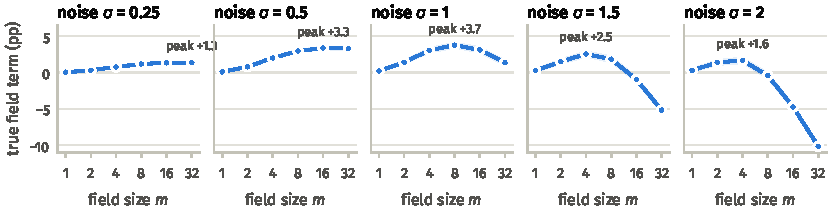
\includegraphics{t0_field_growth}\par
  \vspace{1mm}\raggedright
  \begin{enumerate}
    \item \textbf{The field-term estimator reads high}: $+0.1$ to $+0.2$\pp when the truth is
          zero, $+3.3$\pp when the truth is $+1.6$\pp \ci{+0.4, +2.7}.
    \item \textbf{Fixed effects do not fully clean $\beta_z$} under context dependence:
          $+0.062$ \ci{+0.001, +0.126}.
    \item \textbf{Shared errors give a negative field term with a positive $\beta_z$}. The
          true field term is not monotone in $m$: it peaks at $m = 4$–8 once noise is large
          and is negative at $m = 32$ for $\sigma \geq 1.5$.
  \end{enumerate}
\end{frame}

% ================================================================ 14 eval 3: determinism
\begin{frame}{Evaluation 3: the traces are deterministic, so the floor is zero}
  \framesubtitle{Five repeats of the 20-document pilot: 4-bit on one GPU, and fp16 across two}
  \vspace{5mm}
  \begin{columns}[T,onlytextwidth]
    \begin{column}{0.22\textwidth}
      \stat{0}{non-determinism floor: repeats are bitwise identical in $\ell$, agreement
        and $\Delta(m)$}
    \end{column}
    \begin{column}{0.22\textwidth}
      \stat{1,480}{forward passes in the T2 pilot: 192,088 position rows in 195\,s}
    \end{column}
    \begin{column}{0.22\textwidth}
      \stat{7.6/s}{256-token forward passes, LLaDA-8B in fp16 split over 2 × RTX 2080 Ti}
    \end{column}
    \begin{column}{0.22\textwidth}
      \stat{$\approx$34\,h}{per 2,000-document arm under the full design (466 passes per
        document)}
    \end{column}
  \end{columns}
  \vspace{8mm}
  \begin{takeaway}
    With a zero floor, the ``twice the floor'' bar is met by any nonzero effect, so the
    pre-registered $\delta_{\min} = 2$\pp governs power. Turing GPUs have no bfloat16, so the
    8B models run in fp16 over two GPUs, and every pass is checked for inf/NaN logits.
  \end{takeaway}
\end{frame}

% ================================================================ 15 eval 4: T2 calibration
\begin{frame}{Evaluation 4 (T2 pilot): LLaDA-8B-Base is close to calibrated}
  \framesubtitle{20 reserve documents in fp16: uniform masks at rates 0.1–0.9, plus a top-4 teacher-forced trajectory}
  \vspace{1mm}
  \begin{columns}[T,onlytextwidth]
    \begin{column}{0.42\textwidth}
      \centering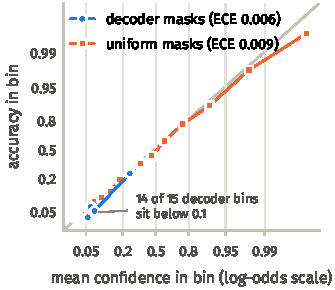
\includegraphics{t2_reliability}
    \end{column}
    \begin{column}{0.56\textwidth}
      \vspace{1mm}
      \footnotesize
      \renewcommand{\arraystretch}{1.1}
      \arrayrulecolor{base}
      \begin{tabularx}{\linewidth}{@{}L r r@{}}
        \toprule
        {\color{ink2}pp unless noted} & {\color{ink2}Decoder} & {\color{ink2}Uniform} \\
        \midrule
        States                     & 1,280 & 200 \\
        ECE                        & 0.6 & 0.9 \\
        $\Delta(1)$, $\Delta(32)$  & 0.6, 1.1 & 0.7, 0.9 \\
        $\Delta(32) - \Delta(1)$   & +0.5 \ci{−0.9, +1.9} & +0.2 \ci{−0.8, +1.2} \\
        Field(32) $-$ field(1)     & −0.04 \ci{−0.14, +0.07} & +0.62 \ci{+0.52, +0.72} \\
        Residual ICC (ratio)       & 0.007 & 0.005 \\
        $\sigma_d$ of the contrast & 3.2 & 2.3 \\
        \bottomrule
      \end{tabularx}
      \vspace{2.5mm}
      \begin{itemize}
        \item Bins hug the diagonal in both arms. Decoder positions sit at low confidence
              because most decoder states are heavily masked.
      \end{itemize}
    \end{column}
  \end{columns}
\end{frame}

% ================================================================ 16 T2 gap
\begin{frame}{T2: the committed-token gap does not grow with field size}
  \vspace{1mm}
  \centering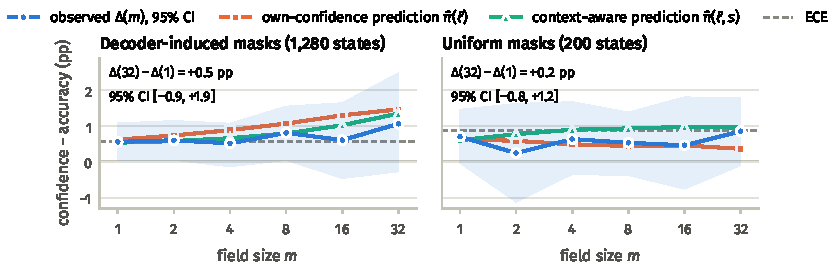
\includegraphics{t2_gap}\par
  \vspace{1.5mm}\raggedright
  \begin{columns}[T,onlytextwidth]
    \begin{column}{0.485\textwidth}
      \begin{itemize}
        \item $\Delta(m)$ stays within 0.2–1.1\pp at every $m$: \textbf{no E1 effect}. The
              decoder interval tops out at $+1.9$\pp, just under $\delta_{\min} = 2$\pp.
      \end{itemize}
    \end{column}
    \begin{column}{0.485\textwidth}
      \begin{itemize}
        \item The uniform field contrast ($+0.6$\pp) excludes zero but is a third of
              $\delta_{\min}$, and T0 says the estimator reads high: a calibrator-refit
              bootstrap will check it.
      \end{itemize}
    \end{column}
  \end{columns}
\end{frame}

% ================================================================ 17 T2 diagnostics
\begin{frame}{T2 diagnostics: the decoder arm carries T0's shared-error signature}
  \framesubtitle{Eq.~2 ($\beta_z$) and Eq.~3 (rank dummies $\gamma_k$) on winning tokens; pooled fit on 20 documents}
  \vspace{1mm}
  \centering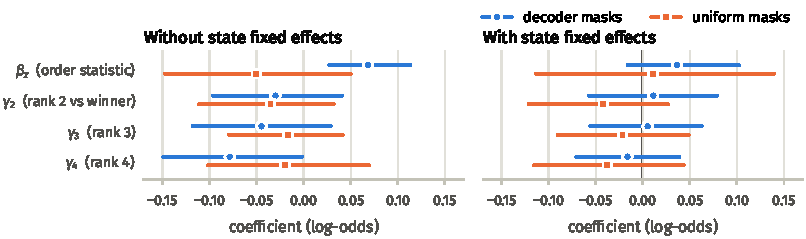
\includegraphics{t2_forest}\par
  \vspace{1.5mm}\raggedright
  \begin{columns}[T,onlytextwidth]
    \begin{column}{0.485\textwidth}
      \begin{itemize}
        \item Decoder arm: $\beta_z$ without FE is \textbf{positive}, $+0.069$
              \ci{+0.027, +0.113}, shrinking with FE; residual ICC 0.007
              \ci{0.004, 0.010}: T0's row four.
      \end{itemize}
    \end{column}
    \begin{column}{0.485\textwidth}
      \begin{itemize}
        \item At equal confidence, rank 4 is less accurate than the winner:
              $\gamma_4 = -0.079$ \ci{−0.149, −0.002}. \textbf{Exploratory}: one of three
              $\gamma_k$, uncorrected.
      \end{itemize}
    \end{column}
  \end{columns}
\end{frame}

% ================================================================ 18 precision
\begin{frame}{Committed tokens, and why precision is in the controls table}
  \vspace{2mm}
  \begin{columns}[T,onlytextwidth]
    \begin{column}{0.48\textwidth}
      \centering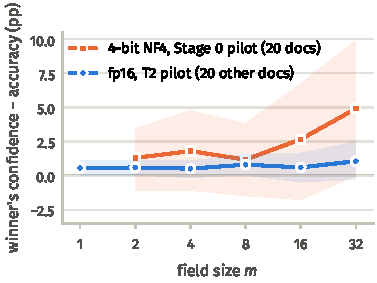
\includegraphics{precision}\par
      \vspace{0.5mm}\raggedright
      \fnote{Pool winners, decoder masks. The pilots also differ in documents and pool
      design: a reason to test, not a result.}
    \end{column}
    \begin{column}{0.49\textwidth}
      \vspace{1mm}
      \begin{itemize}
        \item \textbf{Tokens the top-4 decoder actually committed} (fp16) are overconfident
              by 1.0 to 2.0\pp when 32 to 128 positions remain masked; every interval
              includes zero.
        \item \textbf{The proposal-era Stage 0 pilot}, with 4-bit NF4 weights, put winners
              at 1.2 to 4.9\pp; at $m = 32$ that is 4.9\pp against 1.1\pp in fp16.
        \item So \textbf{4-bit against fp16 on 200 documents} heads the controls ablation
              (T8), beside the PC-Sampler weight, position, token type and a per-step
              temperature.
      \end{itemize}
    \end{column}
  \end{columns}
\end{frame}

% ================================================================ 19 power
\begin{frame}{Evaluation 5: the full sample can see effects of about 0.3 points}
  \vspace{2mm}
  \begin{columns}[T,onlytextwidth]
    \begin{column}{0.5\textwidth}
      \centering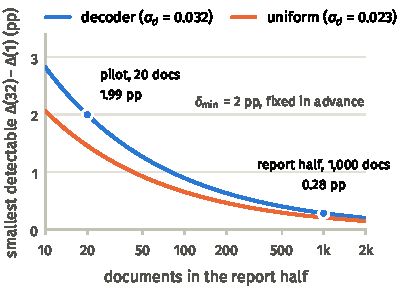
\includegraphics{power}\par
      \vspace{0.5mm}\raggedright
      \fnote{80\% power, two-sided 5\%: $n = 7.85\,\sigma_d^2/\delta^2$, with $\sigma_d$ the
      between-document s.d.\ of the contrast in the pilot.}
    \end{column}
    \begin{column}{0.47\textwidth}
      \vspace{1mm}
      \begin{itemize}
        \item With the pilot's $\sigma_d = 0.032$, 20 documents already reach
              $\delta_{\min}$.
        \item A \textbf{1,000-document report half} gives a standard error of about
              0.1\pp on the contrast: effects near \textbf{0.3\pp} are detectable.
      \end{itemize}
      \vspace{2.5mm}
      \begin{takeaway}
        \textbf{Gate G1}, written and committed before the sweep: required $N = 20 \leq
        1{,}000$, so \textbf{run the full plan}. Binding endpoint: the decoder-arm contrast.
      \end{takeaway}
    \end{column}
  \end{columns}
\end{frame}

% ================================================================ 20 110M
\begin{frame}{Evaluation 6: our 110M masked diffusion LM}
  \framesubtitle{Trained on FineWeb-Edu with our 2,000 calibration documents held out}
  \vspace{1.5mm}
  \begin{columns}[T,onlytextwidth]
    \begin{column}{0.43\textwidth}
      \footnotesize
      \renewcommand{\arraystretch}{1.08}
      \arrayrulecolor{base}
      \begin{tabularx}{\linewidth}{@{}l L@{}}
        \toprule
        Model     & bidirectional transformer: 12 layers, width 768, 12 heads, learned positions \\
        Tokens    & GPT-2 BPE + [MASK]; sequence length 256 \\
        Objective & MDLM (weighted masked cross-entropy) \\
        Optimiser & AdamW, lr $3{\times}10^{-4}$, 2,000 warm-up, decay to 10\%, EMA 0.9999, fp16 \\
        v1 run    & 76,293 steps × 131,072 tokens = 10.0B tokens \\
        \bottomrule
      \end{tabularx}
    \end{column}
    \begin{column}{0.54\textwidth}
      \begin{columns}[T,onlytextwidth]
        \begin{column}{0.48\textwidth}
          \begin{panel}[colback=wash, colframe=wash, height=22mm]
            \stat{38.4}{perplexity \emph{bound} (NELBO) on the 2,000 held-out docs
              \ci{37.7, 39.2}}
          \end{panel}
        \end{column}
        \begin{column}{0.48\textwidth}
          \begin{panel}[height=22mm]
            \stat{28.5}{GPT-2 small (124M), \emph{exact} perplexity, same docs
              \ci{28.0, 29.0}}
          \end{panel}
        \end{column}
      \end{columns}
      \vspace{1.5mm}
      {\footnotesize\raggedright An expected gap: MDLM gives only an upper bound, and GPT-2
      saw other data with far more compute. The fair reference is a same-size AR model on our
      data, trained by the same code.\par}
      \vspace{1.5mm}
      {\footnotesize\raggedright\textbf{Sample}: locally fluent, globally incoherent.
      {\color{ink2}\itshape ``Maintain aeration while the protects food and bottom
      packaging wastes.''}\par}
    \end{column}
  \end{columns}
  \src{The v2 run, trained against the v2 exclusion record, stopped on 29 Sep at step 11,500
  (about 0.7B of 10B tokens). Its retraining, evaluation and gate G2 are still open.}
\end{frame}

% ================================================================ 21 section
\sectionslide{STATUS AND PLAN}{Where each task stands}{%
  What is done, what we got wrong, and the path to the final submission on 31~October}

% ================================================================ 22 status
\begin{frame}{Status by task at the mid submission}
  \vspace{1.5mm}
  \scriptsize
  \renewcommand{\arraystretch}{1.12}
  \arrayrulecolor{base}
  \begin{tabularx}{\linewidth}{@{}p{2.75cm} p{1.75cm} L L@{}}
    \toprule
    {\color{ink2}Task} & {\color{ink2}Status} & {\color{ink2}What exists} & {\color{ink2}Remaining} \\
    \midrule
    Stage 0 (proposal era) & \hb{1} done          & LLaDA-8B 4-bit, 20 docs; both gates recorded & superseded by T2 \\
    T0 theory, simulations & \hb{0.75} mostly     & Propositions 1–2; four-world table and figure & second-person proof check; gate G0 \\
    T1 trace pipeline      & \hb{1} done          & schema v2, three mask kinds, sharded and resumable; floor 0 & — \\
    T2 pilot, power        & \hb{0.75} mostly     & LLaDA-8B-Base fp16 pilot; gate G1 = full plan & split manifest; freeze pre-registration \\
    T3 110M model          & \hb{0.5} partly      & v1 trained and evaluated; AR reference code & v2 retrain and evaluation, G2, AR run, release \\
    T4 contamination       & \hb{0.5} partly      & screens on both 8B base models & pre-register threshold; time-split set \\
    T5–T7 E1, E2, E3       & \hb{0} not started   & estimators, calibrators, pilot numbers & full 2,000-document sweep \\
    T8 controls            & \hb{0} not started   & precision adapters; PC-Sampler weight & precision, position, token type, temperature \\
    T9–T10 C2              & \hb{0} not started   & fine-tuning hook; $p$(true) and top-20 in traces & probe generator, exact terms, real-text proxy \\
    T11–T12 C3, decoders   & \hb{0.5} partly      & decode loop, six commit policies; tasks formatted & recalibration rule; task runs \\
    \bottomrule
  \end{tabularx}
\end{frame}

% ================================================================ 23 challenges
\begin{frame}{Challenges and deviations}
  \vspace{2mm}
  \begin{columns}[T,onlytextwidth]
    \begin{column}{0.485\textwidth}
      \begin{panel}[height=54mm]
        \paneltitle{Identification and estimation}
        \begin{itemize}\footnotesize
          \item The largest change is conceptual: Proposition 1 broke the proposal's
                heteroskedasticity argument, and T0 showed $\beta_z$ with fixed effects
                cannot see the field term. We reframed before any GPU time.
          \item The spline control can create a spurious $\beta_z$ up to $+0.12$, so the
                knots are now fixed in advance.
          \item The field-term estimator reads about twice the truth, and E2 intervals still
                treat fitted calibrators as fixed.
        \end{itemize}
      \end{panel}
    \end{column}
    \begin{column}{0.485\textwidth}
      \begin{panel}[height=54mm]
        \paneltitle{Compute and infrastructure}
        \begin{itemize}\footnotesize
          \item RTX 2080 Ti only (11\,GB, no bfloat16): 8B models in fp16 over two GPUs,
                about 34\,h per 2,000-document arm.
          \item Full-plan traces with top-20 fp32 probabilities need about 83\,GB, more than
                the 76\,GB free; top-10 needs 53\,GB.
          \item Shared storage is not mounted on compute nodes; jobs stage data over ssh.
          \item The 110M v2 run stopped at step 11,500 and must be retrained; the
                pre-registration is not frozen yet.
        \end{itemize}
      \end{panel}
    \end{column}
  \end{columns}
\end{frame}

% ================================================================ 24 plan
\begin{frame}{Path to the final submission}
  \framesubtitle{The C1 sweep is the critical path; the JSON probe is built in parallel so C2 does not wait}
  \vspace{4mm}
  \centering
  \begin{tikzpicture}[
      stp/.style={draw=base, line width=0.5pt, rounded corners=1.5pt, fill=white,
        text width=4.18cm, minimum height=1.36cm, align=left, inner sep=1.5mm,
        font=\scriptsize, text=ink2},
      crit/.style={stp, fill=wash, draw=accent!55},
      num/.style={font=\footnotesize\firasemibold, text=accentdark},
      arr/.style={-{Stealth[length=1.5mm]}, line width=0.6pt, color=muted},
      node distance=3.6mm]
    \node[crit] (s1) {{\footnotesize\firasemibold\color{ink} Freeze and retrain}\\pre-registration (split manifest, contamination threshold, analysis config); gate G0; 110M v2 and gate G2};
    \node[crit, right=of s1] (s2) {{\footnotesize\firasemibold\color{ink} C1 trace sweep}\\2,000 docs on the 110M (fp32) and both 8B base models (fp16), all mask kinds; Instruct on GSM8K, MBPP};
    \node[crit, right=of s2] (s3) {{\footnotesize\firasemibold\color{ink} Primary analysis}\\report half; knot sensitivity panel; with and without flagged docs; calibrator-refit E2 intervals};
    \node[stp, below=7mm of s1] (s4) {{\footnotesize\firasemibold\color{ink} Controls (T8)}\\one ablation table: 4-bit vs fp16 on 200 docs, PC-Sampler weight, position, token type, temperature};
    \node[stp, right=of s4] (s5) {{\footnotesize\firasemibold\color{ink} C2 on the JSON probe}\\$\rho \in \{0, .25, \dots, 1\}$ × $k \in \{1,2,4,8\}$; (A)+(B) must match the direct KL to $10^{-6}$ nats; then 300 real docs};
    \node[stp, right=of s5] (s6) {{\footnotesize\firasemibold\color{ink} C3 and decoders}\\context-aware threshold vs six decoders on GSM8K and MBPP at matched tokens per step; nulls reported};
    \foreach \n/\k in {s1/1,s2/2,s3/3,s4/4,s5/5,s6/6}
      \node[num, anchor=north east] at ([xshift=-1.1mm,yshift=-0.9mm]\n.north east) {\k};
    \draw[arr] (s1) -- (s2); \draw[arr] (s2) -- (s3);
    \draw[arr] (s3.south) -- ++(0,-3.4mm) -| (s4.north);
    \draw[arr] (s4) -- (s5); \draw[arr] (s5) -- (s6);
    \node[anchor=south west, font=\tiny\firasemibold, text=accentdark, inner sep=0.8mm] at (s1.north west) {CRITICAL PATH};
  \end{tikzpicture}
  \par\vspace{4mm}\raggedright
  \begin{takeaway}
    Then the paper, viva slides, and release of the traces and the 110M checkpoint for the
    final submission on 31 October.
  \end{takeaway}
\end{frame}

% ================================================================ 25 summary
\begin{frame}{Summary}
  \vspace{2mm}
  \begin{columns}[T,onlytextwidth]
    \begin{column}{0.485\textwidth}
      \begin{panel}[height=25mm]
        \paneltitle{1 · The question is sharper than proposed}
        Selection alone cannot bias a calibrated posterior (Proposition 1). Any bias lives
        in the field term (Proposition 2), which the instrument measures directly.
      \end{panel}
      \vspace{1.5mm}
      \begin{panel}[height=25mm]
        \paneltitle{2 · The instrument works on known truth}
        The endpoints separate four simulated worlds where ECE cannot. Known weaknesses are
        fixed in advance (9 knots) or flagged (the field estimator reads high).
      \end{panel}
    \end{column}
    \begin{column}{0.485\textwidth}
      \begin{panel}[height=25mm]
        \paneltitle{3 · First real model: near-calibrated, no gradient}
        LLaDA-8B-Base fp16: ECE 0.6\pp and $\Delta(32) - \Delta(1) = +0.5$\pp
        \ci{−0.9, +1.9}. The decoder arm shows a shared-error signature.
      \end{panel}
      \vspace{1.5mm}
      \begin{panel}[height=25mm]
        \paneltitle{4 · Ready to scale}
        Deterministic traces, a written G1 gate, and a design that detects 0.3-point effects.
        Next: the 2,000-document sweep on three models, then C2 and C3.
      \end{panel}
    \end{column}
  \end{columns}
\end{frame}

% ================================================================ 26 thanks
\begin{frame}[c,plain]
  \hspace*{4mm}\begin{minipage}{0.86\linewidth}\raggedright
    {\fontsize{24}{28}\selectfont\firasemibold Thank you. Questions?}\par
    \vspace{3mm}
    {\color{accent}\rule{14mm}{1.6pt}}\par
    \vspace{4mm}
    \small\color{ink2}
    \begin{tabular}{@{}ll@{}}
      Weights \& Biases & wandb.ai/ANLP-project/c3-dllm-calibration \\
      Hugging Face      & huggingface.co/ANLP-project \\
      Mid report        & DuckDuckDuckGoose-Mid.pdf \\
    \end{tabular}
  \end{minipage}
\end{frame}

% ================================================================ backup
\appendix

\begin{frame}{Backup: proofs}
  \framesubtitle{$W_i$: the event that $i \in P$ wins, $i = \arg\max_{j\in P}\ell_j$; ties broken by independent randomness $U$}
  \vspace{1.5mm}
  \footnotesize
  \begin{columns}[T,onlytextwidth]
    \begin{column}{0.485\textwidth}\raggedright
      \paneltitle{Proposition 1}
      Suppose, given $s$, each pair $(\ell_i, a_i)$ is independent of
      $\ell_{-i} = (\ell_j)_{j \in M\setminus\{i\}}$. Let $Z = (\ell_i, s)$ and
      $Y = (\ell_{-i}, P, U)$.\par\vspace{1mm}
      Given $s$, $(\ell_i, a_i) \perp \ell_{-i}$ and $(P, U) \perp (\ell_j, a_j)_{j\in M}$, so
      $(\ell_i, a_i) \perp Y \mid s$, and by weak union $a_i \perp Y \mid Z$, i.e.\
      $\mathbb{E}[a_i \mid Y, Z] = \pi(\ell_i, s)$.\par\vspace{1mm}
      $W_i$ is determined by $(Y, Z)$, so for every bounded measurable $h$
      \[
        \mathbb{E}[a_i h(Z) \mathbb{1}_{W_i}] = \mathbb{E}[\pi(\ell_i, s) h(Z) \mathbb{1}_{W_i}].
      \]
      Dividing by $\Pr(W_i) > 0$ gives $\mathbb{E}[a_i \mid Z, W_i] = \pi(\ell_i, s)$ a.s.
    \end{column}
    \begin{column}{0.485\textwidth}\raggedright
      \paneltitle{Proposition 2}
      Exactly one $W_i$ holds. Applying the display with $h \equiv 1$, summing over $i$ and
      averaging over $s$:
      \[
        \mathbb{E}_m[a] = \textstyle\sum_i \mathbb{E}_m[a_i \mathbb{1}_{W_i}]
        = \textstyle\sum_i \mathbb{E}_m[\pi(\ell_i, s)\mathbb{1}_{W_i}]
        = \mathbb{E}_m[\pi(\ell, s)],
      \]
      so $\Delta(m) = \mathbb{E}_m[\sigma(\ell) - \pi(\ell, s)]$; add and subtract
      $\pi(\ell)$.\par\vspace{1mm}
      At $m = 1$, $\mathbb{E}_1[\pi(\ell)] = \mathbb{E}_1[a]$ by the tower property and
      $\mathbb{E}_1[\pi(\ell, s)] = \mathbb{E}_1[a]$ by the display, so the field term is 0.
    \end{column}
  \end{columns}
\end{frame}

\begin{frame}{Backup: T2 pilot, full table}
  \framesubtitle{LLaDA-8B-Base fp16, 20 documents; probability units as in the report; 95\% document-bootstrap intervals}
  \vspace{1.5mm}
  \centering
  \footnotesize
  \renewcommand{\arraystretch}{1.06}
  \arrayrulecolor{base}
  \begin{tabular}{@{}l r r@{}}
    \toprule
    & {\color{ink2}Decoder} & {\color{ink2}Uniform} \\
    \midrule
    States                        & 1,280 & 200 \\
    ECE                           & 0.006 & 0.009 \\
    $\Delta(1)$                   & 0.006 & 0.007 \\
    $\Delta(32)$                  & 0.011 & 0.009 \\
    $\Delta(32) - \Delta(1)$      & +0.005 \ci{−0.009, 0.019} & +0.002 \ci{−0.008, 0.012} \\
    Field(32) $-$ field(1)        & −0.0004 \ci{−0.0014, 0.0007} & +0.006 \ci{0.005, 0.007} \\
    $\beta_z$, no FE              & +0.069 \ci{0.027, 0.113} & −0.050 \ci{−0.148, 0.050} \\
    $\beta_z$, with FE            & +0.037 \ci{−0.016, 0.102} & +0.011 \ci{−0.114, 0.140} \\
    Residual ICC                  & 0.007 & 0.005 \\
    $\sigma_d$ of contrast        & 0.032 & 0.023 \\
    Documents for 80\% power      & 20 & 11 \\
    \bottomrule
  \end{tabular}
\end{frame}

\begin{frame}{Backup: what the traces cost}
  \framesubtitle{Schema v2, per 256-token document; bytes measured on LLaDA-8B rows}
  \vspace{2mm}
  \begin{columns}[T,onlytextwidth]
    \begin{column}{0.5\textwidth}
      \footnotesize
      \renewcommand{\arraystretch}{1.1}
      \arrayrulecolor{base}
      \begin{tabularx}{\linewidth}{@{}L r r@{}}
        \toprule
        {\color{ink2}Design} & {\color{ink2}Rows} & {\color{ink2}Passes} \\
        \midrule
        Full plan v2              & 60,390 & 466 \\
        Without matched uniform   & 31,334 & 242 \\
        T2 pilot preset           & 9,601  & 74 \\
        \bottomrule
      \end{tabularx}
      \vspace{3mm}
      \begin{tabularx}{\linewidth}{@{}L r r@{}}
        \toprule
        {\color{ink2}Stored top-$k$} & {\color{ink2}Bytes per row} & {\color{ink2}Full plan} \\
        \midrule
        top-20, fp32 probabilities & 186 & 83\,GB \\
        top-10, fp32 probabilities & 117 & 53\,GB \\
        \bottomrule
      \end{tabularx}
    \end{column}
    \begin{column}{0.46\textwidth}
      \begin{itemize}
        \item Every masked position stores $v_i$, $c_i$, $\ell_i$, $a_i$, the true token's
              probability, entropy, margin, the top-20 ids and probabilities, the change in
              $\ell_i$ since the previous step, and the commit rank.
        \item The top-$k$ list is more than 80\% of the bytes.
        \item Bytes were measured on a toy whose top-20 below the true token is noise: an
              upper bound for real models.
      \end{itemize}
    \end{column}
  \end{columns}
\end{frame}

\begin{frame}{Backup: references}
  \vspace{1.5mm}
  \scriptsize
  \setlength{\parskip}{2.4pt}
  \raggedright\color{ink2}
  Andrews, Kitagawa \& McCloskey (2024). Inference on winners. \emph{Quarterly Journal of Economics} 139(1).\par
  Austin et al.\ (2021). Structured denoising diffusion models in discrete state-spaces. \emph{NeurIPS}.\par
  Chang et al.\ (2022). MaskGIT: masked generative image transformer. \emph{CVPR}.\par
  Cobbe et al.\ (2021). Training verifiers to solve math word problems. arXiv:2110.14168.\par
  Efron (2011). Tweedie's formula and selection bias. \emph{JASA} 106(496).\par
  Frkovic et al.\ (2026). Re-evaluating confidence remasking in masked diffusion language models. arXiv:2606.12232.\par
  Guo et al.\ (2017). On calibration of modern neural networks. \emph{ICML}.\par
  Jazbec et al.\ (2026). Learning unmasking policies for diffusion language models. \emph{ICML}.\par
  Kang et al.\ (2026). ParallelBench: understanding the trade-offs of parallel decoding in diffusion LLMs. \emph{ICLR}.\par
  Olausson et al.\ (2026). A tale of two temperatures: sampling from diffusion language models. arXiv:2604.09921.\par
  Penedo et al.\ (2024). The FineWeb datasets: decanting the web for the finest text data at scale. arXiv:2406.17557.\par
  Sahoo et al.\ (2024). Simple and effective masked diffusion language models. \emph{NeurIPS}.\par
  Tang et al.\ (2026). Is your diffusion sampler actually correct? \emph{ICML}.\par
  Wu et al.\ (2025). Fast-dLLM: training-free acceleration of diffusion LLM. arXiv:2505.22618.\par
\end{frame}

\end{document}
